% !TeX root = surprises.tex


\selectlanguage{hebrew}


\chapter{אפשר להסתפק בסרגל ביחד עם מעגל אחד}\label{c.straightedge}

%%%%%%%%%%%%%%%%%%%%%%%%%%%%%%%%%%%%%%%%%%%%%%%%%%%%%%%%%%%%%%%


האם כל בניה עם סרגל ומחוגה ניתנת לבניה עם סרגל בלבד? התשובה היא שלילית. ב-%
$1822$
\L{Jean-Victor Poncelet}
שיער שכן ניתן להסתפק בסרגל בלבד בתנאי שקיים במישור מעגל אחד.
המשפט הוכח ב-%
$1833$
על ידי
\L{Jakob Steiner}.

%%%%%%%%%%%%%%%%%%%%%%%%%%%%%%%%%%%%%%%%%%%%%%%%%%%%%%%%%%%%%%%


כל צעד בבניה עם סרגל ומחוגה הוא אחת משלושת הפעולות הללו:
\begin{itemize}
\setlength{\itemsep}{0pt}
\item
מציאת נקודת החיתוך של שני קווים.
\item
מציאת נקודות החיתוך של קו עם מעגל.
\item
מציאת נקודות החיתוך של שני מעגלים.
\end{itemize}
ברור שניתן לבצע את הפעולה הראשונה עם סרגל בלבד. עלינו להראות שעבור שתי הפעולות האחרות ניתן למוצא בניה שקולה שמשתמשת רק בסרגל עם מעגל אחד.

%%%%%%%%%%%%%%%%%%%%%%%%%%%%%%%%%%%%%%%%%%%%%%%%%%%%%%%%%%%%%%%

מה המשמעות של בניה עם סרגל בלבד? מעגל מוגדר על ידי נקודה
$O$,
שהיא מרכז המעגל, וקטע קו באורך
$r$,
הרדיוס, שאחת מהנקודות הקצה שלו היא
$O$.
אם נצליח לבנות את הנקודות
$X,Y$
המסומנות באיור שלהלן, נוכל לטעון שהצלחנו לבנות את נקודות החיתוך של מעגל נתון עם קו נתון ושל שני מעגלים נתונים. בהמשך, המעגל הנתון יצוייר בקו רגיל והמעגלים שמשמשים רק להדגמת הבניה יצויירו מקווקווים.
\begin{center}

\begin{tikzpicture}[scale=.9]
\fill (0,0) node[above right] {$O$} circle[radius=1.5pt];
\draw[thick,dashed,name path=circle] (0,0) circle[radius=2cm];
\draw (0,0) -- node[left] {$r$} ++(-60:2cm);
\fill (0,0) ++(-60:2cm) circle[radius=1.5pt];
\draw[name path=line] (-3,-.5) -- ++(20:6cm);
\path [name intersections={of=circle and line,by={X,Y}}];
\fill (X) node[above right,xshift=-2pt,yshift=4pt] {$X$} circle[radius=1.5pt];
\fill (Y) node[above left] {$Y$} circle[radius=1.5pt];
\begin{scope}[xshift=6cm]
\fill (0,0) node[above right] {$O_1$} circle[radius=1.5pt];
\fill (3,0) node[above right] {$O_2$} circle[radius=1.5pt];
\draw[thick,dashed,name path=circle1] (0,0) circle[radius=2cm];
\draw[thick,dashed,name path=circle2] (3,0) circle[radius=2cm];
\draw (0,0) -- node[left] {$r_1$} ++(-70:2cm);
\draw (3,0) -- node[left,below] {$r_2$} ++(-20:2cm);
\fill (0,0) ++(-70:2cm) circle[radius=1.5pt];
\fill (3,0) ++(-20:2cm) circle[radius=1.5pt];
\path [name intersections={of=circle1 and circle2,by={X,Y}}];
\fill (X) node[above,yshift=4pt] {$X$} circle[radius=1.5pt];
\fill (Y) node[below,yshift=-4pt] {$Y$} circle[radius=1.5pt];
\end{scope}
\end{tikzpicture}
\end{center}
%%%%%%%%%%%%%%%%%%%%%%%%%%%%%%%%%%%%%%%%%%%%%%%%%%%%%%%%%%%%%%%
תחילה נביא חמש בניות עזר נחוצות )סעיפים
\ref{s.parallel}--\ref{s.root}%
(,
ואחר כך נראה איך למצוא את נקודות החיתוך של קו עם מעגל )סעיף
\ref{s.line-circle-straight}(
ושל שני מעגלים )סעיף
\ref{s.circle-circle}(.


%%%%%%%%%%%%%%%%%%%%%%%%%%%%%%%%%%%%%%%%%%%%%%%%%%%%%%%%%%%%%%%


\selectlanguage{hebrew}


\section{%
בניית קו המקביל לקו נתון%
}\label{s.parallel}

\begin{theorem}\label{thm.parallel-line}\mbox{}\\
נתון קו
$l$
העובר דרך שתי נקודות
$A,B$,
ונתונה נקודה 
$P$
)שאיננה על הקו(, ניתן לבנות קו דרך
$P$
המקביל ל-%
$\overline{AB}$.
\end{theorem}
\textbf{הוכחה:}
נפריד את הבניה לשני מקרים:
\begin{enumerate}
\item
"קו מכוון": נתונה גם הנקודה
$M$
שהיא נקודת האמצע של קטע הקו
$\overline{AB}$.
\item
כל קו אחר.
\end{enumerate}



\textbf{מקרה ראשון:}
בנו קרן הממשיכה את
$\overline{AP}$,
ובחרו
$S$,
נקודה כלשהי על הקרן מעבר ל-%
$P$.
בנו את הקווים
$\overline{SB}$, $\overline{SM}$, $\overline{BP}$.
סמנו ב-%
$O$
את נקודת החיתוך של 
$\overline{BP}$
עם
$\overline{SM}$.
בנו קרן הממשיכה את
$\overline{AO}$
וסמנו ב-%
$Q$
את החיתוך של הקרן עם
$\overline{SB}$.
\begin{center}

\vspace*{-4pt}
\begin{tikzpicture}
\draw[name path=pq] (-4,0) -- (4,0);
\draw (-2,-2) node[below left] {$A$} coordinate (A) -- (2,-2) node[below right] {$B$} coordinate (B);
\fill (A) circle[radius=1.5pt];
\fill (B) circle[radius=1.5pt];
\draw[name path=as] (A) -- ++(50:4cm) node[above] {$S$} coordinate (S);
\fill (S) circle[radius=1.5pt];
\draw[name path=sb] (S) -- (B);
\path [name intersections={of=pq and as,by={P}}];
\path [name intersections={of=pq and sb,by={Q}}];
\fill (P) node[above left] {$P$} circle[radius=1.5pt];
\fill (Q) node[above right] {$Q$} circle[radius=1.5pt];
\draw[name path=pb] (P) -- (B);
\draw[name path=qa] (Q) -- (A);
\path [name intersections={of=pb and qa,by={O}}];
\fill (O) node[right,xshift=2pt] {$O$} circle[radius=1.5pt];
\fill (0,-2) coordinate (M) node[below right] {$M$} circle[radius=1.5pt];
\draw (S) -- (M);
\end{tikzpicture}
\vspace*{-4pt}
\end{center}

\textbf{%
טענה:
$\overline{PQ}\|\overline{AB}$.}

להוכחת הטענה נשתמש במשפט
\L{Ceva}
שנוכיח בהמשך.

\begin{theorem}[\L{Ceva}]\label{thm.ceva}\mbox{}\\
נתונים שלושה קטעי קו מקודקודי משולש לצלעות הנגדיות שנפגשים בנקודה
$M$
)כמו באיור לעיל, אבל 
$M$
לא בהכרח חוצה את הצלע(. קטעי הצלעות מקיימים את היחס:
\[
\frac{\overline{AM}}{\overline{MB}}\cdot\frac{\overline{BQ}}{\overline{QS}}\cdot\frac{\overline{SP}}{\overline{PA}} = 1\,.
\]
\end{theorem}



\textbf{הוכחה של הטענה:}
בבניה למעלה 
$M$
חוצה את
$\overline{AB}$
ולכן
$\disfrac{\overline{AM}}{\overline{MB}}=1$.
מכאן ש:
\begin{equation}
\frac{\overline{BQ}}{\overline{QS}}=\frac{\overline{PA}}{\overline{SP}}=\frac{\overline{AP}}{\overline{PS}}\,.\label{eq.ceva}
\end{equation}



נוכיח ש-%
$\triangle ABS\sim\triangle PQS$,
ולכן
$\overline{PQ}\|\overline{AB}$
כי
$\angle ABS = \angle PQS$.


\textbf{הוכחה שהמשולשים דומים:}

\begin{eqnarray*}
\overline{BS}&=&\overline{BQ}+\overline{QS}\\
\disfrac{\overline{BS}}{\overline{QS}}&=&\disfrac{\overline{BQ}}{\overline{QS}}+\disfrac{\overline{QS}}{\overline{QS}} = \disfrac{\overline{BQ}}{\overline{QS}}+1\\
\overline{AS}&=&\overline{AP}+\overline{PS}\\
\disfrac{\overline{AS}}{\overline{PS}} &=& \disfrac{\overline{AP}}{\overline{PS}} + \disfrac{\overline{PS}}{\overline{PS}} = \disfrac{\overline{AP}}{\overline{PS}} + 1\\
\disfrac{\overline{BS}}{\overline{QS}}=\disfrac{\overline{BQ}}{\overline{QS}}+1&=&\disfrac{\overline{AP}}{\overline{PS}} + 1=\disfrac{\overline{AS}}{\overline{PS}}\,,
\end{eqnarray*}
כאשר המשוואה האחרונה מתקבלת ממשפט
\ref{thm.ceva}.\qed

\textbf{הוכחה של משפט \L{Ceva}:}
\begin{center}

\vspace*{-4pt}
\begin{tikzpicture}
\path[name path=pq] (-4,0) -- (4,0);
\draw (-2,-2) node[below left] {$A$} coordinate (A) -- (2,-2) node[below right] {$B$} coordinate (B);
\coordinate (M) at (0,-2);
\draw[name path=as] (A) -- ++(50:4cm) node[above] {$S$} coordinate (S);
\draw[name path=sb] (S) -- (B);
\path [name intersections={of=pq and as,by={P}}];
\path [name intersections={of=pq and sb,by={Q}}];
\path[name path=pb] (P) -- (B);
\path[name path=qa] (Q) -- (A);
\path [name intersections={of=pb and qa,by={O}}];
\draw[fill=gray!40] (B) -- (O) -- (Q);
\draw[fill=gray!70] (S) -- (O) -- (Q);
\draw (B) -- (O) -- (A);
\draw (S) -- (O) -- (A);
\draw (A) -- (B) -- (S) -- cycle;
\draw (S) -- (O);
\draw (B) -- (O);
\fill (A) circle[radius=1.5pt];
\fill (B) circle[radius=1.5pt];
\fill (S) circle[radius=1.5pt];
\fill (Q) node[above right] {$Q$} circle[radius=1.5pt];
\fill (O) node[above left] {$O$} circle[radius=1.5pt];
\path[name path=al1] (O) -- ($(Q)!(O)!(B)$);
\draw[rotate=-155] ($(Q)!(O)!(B)$) rectangle +(7pt,7pt);
\path [name intersections={of=al1 and sb,by={A1}}];
\draw[thick,dashed] (O) -- (A1);
\begin{scope}[xshift=6cm]
\path[name path=pq] (-4,0) -- (4,0);
\draw (-2,-2) node[below left] {$A$} coordinate (A) -- (2,-2) node[below right] {$B$} coordinate (B);
\coordinate (M) at (0,-2);
\draw[name path=as] (A) -- ++(50:4cm) node[above] {$S$} coordinate (S);
\draw[name path=sb] (S) -- (B);
\path [name intersections={of=pq and as,by={P}}];
\path [name intersections={of=pq and sb,by={Q}}];
\draw[name path=pb] (P) -- (B);
\draw[name path=qa] (Q) -- (A);
\path [name intersections={of=pb and qa,by={O}}];
\draw (B) -- (O) -- (Q);
\draw (A) -- (Q) -- (B);
\draw[fill=gray!40] (B) -- (Q) -- (A);
\draw[fill=gray!70] (S) -- (Q) -- (A);
\draw (A) -- (B) -- (S) -- cycle;
\draw (S) -- (O);
\draw (B) -- (O);
\fill (A) circle[radius=1.5pt];
\fill (B) circle[radius=1.5pt];
\fill (S) circle[radius=1.5pt];
\fill (Q) node[above right] {$Q$} circle[radius=1.5pt];
\fill (O) node[above left] {$O$} circle[radius=1.5pt];
\path[name path=al2] (A) -- ($(Q)!(A)!(B)$);
\draw[rotate=-155] ($(Q)!(A)!(B)$) rectangle +(7pt,7pt);
\path [name intersections={of=al2 and sb,by={A2}}];
\draw[thick,dashed] (A) -- (A2);
\end{scope}
\end{tikzpicture}
\vspace*{-6pt}
\end{center}
אם הגבהים של שני משולשים שווים, יחס השטחים שווה ליחס הבסיסים.
%\[
%A_1 = \frac{1}{2}hb_1,\quad A_2 = \frac{1}{2}hb_2, \quad \frac{A_1}{A_2}=\frac{b_1}{b_2}\,.
%\]
הגבהים של המשולשים 
$\triangle BQO, \triangle SQO$
שווים, כמו גם
$\triangle BQA, \triangle SQA$.
לכן:%
\footnote{%
\R{נשתמש בשם המשולש כקיצור לשטחו}.}
\begin{eqnarray}
\frac{\triangle BQO}{\triangle SQO} &=& \frac{\overline{BQ}}{\overline{QS}}\label{eq.ratio-of-areas1}\\
\frac{\triangle BQA}{\triangle SQA} &=& \frac{\overline{BQ}}{\overline{QS}}\,.\label{eq.ratio-of-areas2}
\end{eqnarray}
על ידי חיסור נקבל יחס בין המשולשים המסומנים באפור:
\begin{center}

\vspace*{-4pt}
\begin{tikzpicture}
\path[name path=pq] (-4,0) -- (4,0);
\draw (-2,-2) node[below left] {$A$} coordinate (A) -- (2,-2) node[below right] {$B$} coordinate (B);
\coordinate (M) at (0,-2);
\draw[name path=as] (A) -- ++(50:4cm) node[above] {$S$} coordinate (S);
\draw[name path=sb] (S) -- (B);
\path [name intersections={of=pq and as,by={P}}];
\path [name intersections={of=pq and sb,by={Q}}];
\path[name path=pb] (P) -- (B);
\draw[thick,name path=qa] (Q) -- (A);
\path [name intersections={of=pb and qa,by={O}}];
\draw[fill=gray!50] (B) -- (O) -- (A);
\draw[fill=gray!70] (S) -- (O) -- (A);
\draw (B) -- (O) -- (A);
\draw (S) -- (O) -- (A);
\draw (A) -- (B) -- (S) -- cycle;
\draw (S) -- (O);
\draw (B) -- (O);
\fill (A) circle[radius=1.5pt];
\fill (B) circle[radius=1.5pt];
\fill (S) circle[radius=1.5pt];
\fill (Q) node[above right] {$Q$} circle[radius=1.5pt];
\fill (O) node[right,xshift=2pt] {$O$} circle[radius=1.5pt];
\end{tikzpicture}
\end{center}
\[
\frac{\triangle BQA - \triangle BQO}{\triangle SQA-\triangle SQO} = \frac{\triangle BOA}{\triangle SOA} = \frac{\overline{BQ}}{\overline{QS}}\,.\label{eq.diff-of-areas}
\]
נסביר את החישוב תוך שימוש בסימונים פשוטים יותר:
\[
a=\overline{BQ},\, b=\overline{QS},\,
c=\triangle{BQA},\, d=\triangle{SQA},\,
e=\triangle{BQO},\,f=\triangle{SQO}\,.
\]
מהמשוואות
\ref{eq.ratio-of-areas1}, \ref{eq.ratio-of-areas2}:

\begin{eqnarray}
 \disfrac{c}{d} &=&\disfrac{a}{b}\\
 \disfrac{e}{f} &=&\disfrac{a}{b}\,.
\end{eqnarray}
מחישוב פשוט:

\begin{eqnarray*}
c-e &=& \disfrac{ad}{b} - \disfrac{af}{b}= \disfrac{a}{b}(d-f)\\
\disfrac{c-e}{d-f} &=& \disfrac{a}{b}
\end{eqnarray*}
מתקבלת המשוואה
\ref{eq.diff-of-areas}.

באופן דומה ניתן להוכיח:
\[
\frac{AM}{MB} = \frac{\triangle AOS}{\triangle BOS}\;,\quad\quad \frac{SP}{PA} =\frac{\triangle SOB}{\triangle AOB}\;,
\]

ומכאן:
\[
\frac{AM}{MB}\cdot\frac{BQ}{QS}\cdot\frac{SP}{PA} = \frac{\triangle AOS}{\triangle BOS}\frac{\triangle BOA}{\triangle SOA}\frac{\triangle SOB}{\triangle AOB}=1\,,
\]

כי סדר הקודקודים  לא משנה
$\triangle AOS\!=\!\triangle SOA, \triangle BOA\!=\!\triangle AOB, \triangle SOB\!=\!\triangle BOS$.
\qed
%%%%%%%%%%%%%%%%%%%%%%%%%%%%%%%%%%%%%%%%%%%%%%%%%%%%%%%%%%%%%%%

\medskip

\textbf{מקרה שני:}
נתון הקו
$l$
ונתונה הנקודה
$P$
שאיננה נמצאת על הקו. סמנו את המרכז של המעגל הקבוע ב-%
$O$
והרדיוס שלו ב-%
$r$.
בחרו נקודה
$M$
על הקו 
$l$
ובנו קרן דרך 
$\overline{MO}$
שחותך את המעגל הקבוע ב-%
$U,V$.
\begin{center}

\begin{tikzpicture}[scale=.8]
\coordinate (O) at (0,0);
\fill (O) node[below right] {$O$} circle[radius=1.5pt];
\draw[name path=circle] (O) circle[radius=2cm];
\draw[name path=l] (-4,-3) -- node[above, near end] {$l$} +(9,0);
\path[name path=mo] (-2,-3) coordinate (M) -- ($(-2,-3)!1.65!(O)$);
\fill (M) node[below] {$M$} circle[radius=1.5pt];
\path [name intersections={of=circle and mo,by={V,U}}];
\fill (U) node[below,xshift=2pt,yshift=-4pt] {$U$} circle[radius=1.5pt];
\fill (V) node[right,xshift=4pt] {$V$} circle[radius=1.5pt];
\draw (M) --   (U) -- node[above] {$r$} (O) -- node[above] {$r$} (V);
%\node at (-1.6,1.6) {$c$};
\fill (-4,1) node[above left] {$P$} circle[radius=1.5pt];
\end{tikzpicture}
\vspace*{-8pt}
\end{center}
קו זה הוא
\textbf{%
קו מכוון%
}
כי 
$O$,
מרכז המעגל, חוצה את הקוטר
$\overline{UV}$.
בחרו נקודה שנייה 
$A$
על 
$l$.
לפי הבניה של המקרה הראשון, ניתן לבנות קו המקביל ל-%
$\overline{UV}$
דרך 
$A$.
יש לבחור את
$A$
כך שהקו המקביל חותך את המעגל בשתי נקודות שנסמן
$X,Y$.
\begin{center}

\begin{tikzpicture}[scale=.9]
\coordinate (O) at (0,0);
\fill (O) node[below right] {$O$} circle[radius=1.5pt];
\draw[name path=circle] (O) circle[radius=2cm];
\draw[name path=l] (-4,-3) -- node[above,near end,xshift=24pt] {$l$} +(9,0);
\path[name path=mo] (-2,-3) coordinate (M) -- ($(-2,-3)!1.65!(O)$);
\fill (M) node[below] {$M$} circle[radius=1.5pt];
\path [name intersections={of=circle and mo,by={V,U}}];
\fill (U) node[below,xshift=2pt,yshift=-4pt] {$U$} circle[radius=1.5pt];
\fill (V) node[right,xshift=4pt] {$V$} circle[radius=1.5pt];
\draw (M) -- (V);
\path[name path=ax] (-3,-3) coordinate (A) -- ($(-3,-3)!1.8!(-1,0)$);
\fill (A) node[below] {$A$} circle[radius=1.5pt];
\path [name intersections={of=circle and ax,by={Y,X}}];
\fill (X) node[left] {$X$} circle[radius=1.5pt];
\fill (Y) node[above] {$Y$} circle[radius=1.5pt];
%\node at (-1.6,1.6) {$c$};
\draw (A) -- (Y);
\fill (-4,1) node[above left] {$P$} circle[radius=1.5pt];
\end{tikzpicture}
\vspace*{-6pt}
\end{center}
בנו קוטר
$\overline{XX'}$
וקוטר
$\overline{YY'}$.
בנו קרן מ-%
$X'$
עבור דרך
$Y'$
וסמנו ב-%
$B$
את נקודת החיתוך שלה עם 
$l$.
\begin{center}

\begin{tikzpicture}[scale=.9]
\coordinate (O) at (0,0);
\fill (O) node[below right] {$O$} circle[radius=1.5pt];
\draw[name path=circle] (O) circle[radius=2cm];
\draw[name path=l] (-4,-3) -- node[above,near end,xshift=24pt] {$l$} +(9,0);
\path[name path=mo] (-2,-3) coordinate (M) -- ($(-2,-3)!1.65!(O)$);
\fill (M) node[below] {$M$} circle[radius=1.5pt];
\path [name intersections={of=circle and mo,by={V,U}}];
\fill (U) node[below,xshift=2pt,yshift=-4pt] {$U$} circle[radius=1.5pt];
\fill (V) node[right,xshift=4pt] {$V$} circle[radius=1.5pt];
\draw (M) -- (V);
\path[name path=ax] (-3,-3) coordinate (A) -- ($(-3,-3)!1.8!(-1,0)$);
\fill (A) node[below] {$A$} circle[radius=1.5pt];
\path [name intersections={of=circle and ax,by={Y,X}}];
\fill (X) node[left] {$X$} circle[radius=1.5pt];
\fill (Y) node[above] {$Y$} circle[radius=1.5pt];
%\node at (-1.6,1.6) {$c$};
\draw (A) -- (Y);
\fill (-4,1) node[above left] {$P$} circle[radius=1.5pt];
\path[name path=xo] (X) -- ($(X)!2.2!(O)$);
\path[name intersections={of=circle and xo,by={Xp}}];
\fill (Xp) node[right,xshift=2pt,yshift=-2pt] {$X'$} circle[radius=1.5pt];
\draw (X) -- (Xp);
\path[name path=yo] (Y) -- ($(Y)!2.4!(O)$);
\path[name intersections={of=circle and yo,by={Yp,y}}];
\fill (Yp) node[below right] {$Y'$} circle[radius=1.5pt];
\draw (Y) -- (Yp);
\path[name path=xy] (Xp) -- ($(Xp)!1.6!(Yp)$);
\path[name intersections={of=l and xy,by={B}}];
\fill (B) node[below] {$B$} circle[radius=1.5pt];
\draw (Xp) -- (B);
\draw[thick,dashed,name path=z] (-4,0) -- (4,0) node[above,near end,xshift=40pt] {$l'$};
\path[name intersections={of=ax and z,by={Z}}];
\path[name intersections={of=xy and z,by={Zp}}];
\fill (Z) node[above left] {$Z$} circle[radius=1.5pt];
\fill (Zp) node[below right] {$Z'$} circle[radius=1.5pt];
\end{tikzpicture}
\vspace*{-10pt}
\end{center}
\textbf{%
טענה:%
}
$l$
הוא
\textbf{קו מכוון}.

\textbf{הוכחה:}
$\overline{OX},\overline{OX'},\overline{OY},\overline{OY'}$
הם כולם רדיוסים של המעגל, ו-%
$\angle XOY = \angle X'OY'$
כי הן זוויות קודקודיות. לכן,
$\triangle XOY\cong \triangle X'OY'$
לפי צלע-זווית-צלע. נגדיר )לא נבנה!( קו
$l'\|l$
שחותך את 
$\overline{XY}$
ב-%
$Z$
ושחותך את 
$X',Y'$
ב-%
$Z'$.
$\angle XOZ=\angle X'OZ'$
כי הן זוויות קודקודיות, ולכן
$\triangle XOZ\cong \triangle X'OZ'$
לפי זווית-צלע-זווית. מכאן ש-%
$\overline{ZO}=\overline{OZ'}$. 
$AMOZ$
ו-%
$BMOZ'$
מקביליות ולכן
$\overline{AM}=\overline{ZO}=\overline{OZ'}=\overline{MB}$
ו-%
$M$
חוצה את
$\overline{AB}$.
\qed

לפי הבניה של המקרה הראשון ניתן לבנות את הקו
$l'$
דרך 
$P$
שמקביל ל-%
$l$.
\qed

משפט~%
\ref{thm.parallel-line}
אומר שניתן לבנות 
\textbf{קו}
דרך 
$P$
המקביל ל-%
$\overline{AB}$.
למעשה גם אפשר לבנות
\textbf{קטע קו}
המקביל ל-%
$\overline{AB}$
שאורכו שווה לאורך של
$\overline{AB}$.

\textbf{מסקנה:}
ניתן להעתיק קטע קו מקביל לעצמו כך שקצה אחד יהיה נקודה כלשהי.

\textbf{הוכחה:}
בנו קו דרך
$P$
המקביל ל-%
$\overline{AB}$,
חברו את
$P$
ו-%
$A$,
ובנו קו
$n$
דרך 
$B$
המקביל ל-%
$\overline{AP}$.
$ABQP$
הוא מקבילית ו-%
$\overline{PQ}=\overline{AB}$.
\begin{center}

\begin{tikzpicture}[scale=.7]
\coordinate (A) at (0,0);
\coordinate (B) at (3,0);
\coordinate (P) at (-2,2.5);
\coordinate (Q) at (1,2.5);
\draw ($(P)!-.6!(Q)$) -- node[above,near end,xshift=36pt] {$m$} ($(P)!2.2!(Q)$);
\fill (P) node[above] {$P$} circle[radius=1.5pt];
\fill (Q) node[above right] {$Q$} circle[radius=1.5pt];
\draw ($(A)!-.6!(B)$) -- node[above,near end,xshift=40pt] {$l$} ($(A)!2.5!(B)$);
\fill (A) node[below] {$A$} circle[radius=1.5pt];
\fill (B) node[below left] {$B$} circle[radius=1.5pt];
\draw (A) -- (P);
\draw ($(B)!-.3!(Q)$) -- node[above,near end,xshift=24pt,yshift=-24pt] {$n$} ($(B)!1.4!(Q)$);
\end{tikzpicture}
\end{center}

%%%%%%%%%%%%%%%%%%%%%%%%%%%%%%%%%%%%%%%%%%%%%%%%%%%%%%%%%%%%%%%

\selectlanguage{hebrew}


\section{%
בניית אנך לקו נתון%
}\label{s.perpendicular}

\begin{theorem}\label{thm.perpendicular}\mbox{}\\
נתון קו
$l$
ונקודה
$P$
)שאיננה על הקו( ניתן לבנות אנך ל-%
$l$
דרך
$P$.%
\end{theorem}

\textbf{הוכחה:}
בנו לפי משפט
\ref{thm.parallel-line}
קו
$l'\|l$
החותך את המעגל הקבוע ב-%
$U,V$.
בנו את הקוטר
$\overline{UOU'}$
והמיתר
$\overline{U'V}$.
$\angle UVU'$
היא זווית ישרה כי היא נשענת על קוטר. מכאן ש-%
$\overline{U'V}\perp l'$.
בנו קו מקביל ל-%
$\overline{U'V}$
דרף
$P$
לפי משפט~%
\ref{thm.parallel-line}.\qed
\begin{center}

\begin{tikzpicture}[scale=.8]
\coordinate (O) at (0,0);
\coordinate (P) at (3.5,.6);
%\node at (-1.6,1.6) {$c$};
\draw[name path=circle] (O) circle[radius=2cm];
\draw[name path=l] (-4,-3) -- node[above,near end,xshift=45pt] {$l$} ++(9.5,0);
\draw[name path=lp] (-3,-1) -- node[above,near end,xshift=45pt] {$l'$} ++(7.5,0);
\fill (O) node[above left] {$O$} circle[radius=1.5pt];
\fill (P) node[right] {$P$} circle[radius=1.5pt];
\path[name intersections={of=circle and lp,by={U,V}}];
\fill (U) node[below left] {$U$} circle[radius=1.5pt];
\fill (V) node[below right] {$V$} circle[radius=1.5pt];
\path[name path=d] (U) -- ($(U)!2.3!(O)$);
\path[name intersections={of=circle and d,by={Up}}];
\draw (U) -- (Up);
\fill (Up) node[above right] {$U'$} circle[radius=1.5pt];
\draw (Up) -- (V);
\path[name path=p] (P) -- ++(0,-4);
\draw[name intersections={of=p and l,by={X}}];
\fill (X) circle[radius=1.5pt];
\draw[thick,dashed] (P) -- (X);
\draw ($(U)!.9!(V)$) -- ++(0,.3) -| (V);
\end{tikzpicture}
\vspace*{-8pt}
\end{center}



%%%%%%%%%%%%%%%%%%%%%%%%%%%%%%%%%%%%%%%%%%%%%%%%%%%%%%%%%%%%%%%

\selectlanguage{hebrew}


\section{%
העתקת קטע קו נתון בכיוון נתון%
}\label{s.direction}

\begin{theorem}\label{thm.angle}\mbox{}\\
נתון נקודה
$A$,
קטע קו
$\overline{PQ}$
וזווית
$\theta$,
ניתן לבנות קטע קו
$\overline{AS}=\overline{PQ}$
בכיוון 
$\theta$.
\end{theorem}
\begin{center}

\vspace*{-8pt}
\begin{tikzpicture}[scale=.8]
\coordinate (A) at (0,0);
\coordinate (P) at (1,-1.5);
\coordinate (Q) at (2.5,-1.5);
\draw (P) -- node[below] {$a$} (Q);
\fill (P) node[left] {$P$} circle[radius=1.5pt];
\fill (Q) node[right] {$Q$} circle[radius=1.5pt];
%\coordinate (A1) at (-4,1);
%\draw[thick,dashed] (A1) -- ++(60:3cm) coordinate (H1);
%\draw[thick,dashed] (A1) -- ++(0:3cm);
%\fill (A1) node[left] {$A'$} circle[radius=1.5pt];
%\fill (H1) node[left] {$H'$} circle[radius=1.5pt];
\draw (A) -- node[left] {$a$} ++(60:1.5cm) coordinate (S);
\fill (S) node[above right] {$S$} circle[radius=1.5pt];
\draw[thick,dashed] (A) -- ++(3,0);
\fill (A) node[left] {$A$} circle[radius=1.5pt];
%\node[above right,xshift=4pt] at (A1) {$\theta$};
\node[above right,xshift=4pt] at (A) {$\theta$};
\end{tikzpicture}
%\vspace*{-12pt}
\end{center}
המשמעות של "בכיוון 
$\theta$"
היא שהזווית בין 
$\overline{AS}$
לקו המקביל ל-%
$\overline{PQ}$
דרך
$A$
היא
$\theta$.

בסוף סעיף
\ref{s.parallel}
הראינו שאפשר להעתיק קטע קו מקביל לעצמו. כאן המטרה היא להעתיק את קטע הקו
$\overline{PQ}$
ל-%
$\overline{AS}$,
כך ש-%
$\overline{AS}$
יהיה באותה זווית
$\theta$
יחסית לאותו ציר. באיור
$\overline{PQ}$
נמצא על ציר ה-%
$x$
אבל אין לזה חשיבות.


\textbf{הוכחה:}
נניח שהזווית הנתונה
$\theta$
היא הזווית בין קטע הקו
$\overline{A'H'}$
לקו מקביל ל-%
$\overline{PQ}$
המכיל את
$A'$.
לפי משפט~%
\ref{thm.parallel-line}
ניתן לבנות קטע קו
$\overline{AH}$
כך ש-%
$\overline{AH}\|\overline{A'H'}$,
וקטע קו
$\overline{AK}$
כך ש-%
$\overline{AK}\|\overline{PQ}$
ו-%
$\overline{AK}=\overline{PQ}=a$.
\begin{center}

\vspace*{-4pt}
\begin{tikzpicture}[scale=.8]
\coordinate (A) at (0,0);
\coordinate (P) at (1,-1.5);
\coordinate (Q) at (2.5,-1.5);
\draw (P) -- node[below] {$a$} (Q);
\fill (P) node[left] {$P$} circle[radius=1.5pt];
\fill (Q) node[right] {$Q$} circle[radius=1.5pt];
\coordinate (A1) at (-3,1);
\draw (A1) -- ++(60:3cm) coordinate (H1);
\draw[thick,dashed] (A1) -- ++(0:1.5cm);
\fill (A1) node[left] {$A'$} circle[radius=1.5pt];
\fill (H1) node[left] {$H'$} circle[radius=1.5pt];
\draw (A) -- ++(60:3cm) coordinate (H);
\fill (H) node[left] {$H$} circle[radius=1.5pt];
\draw (A) -- ++(1.5,0) coordinate (K);
\fill (K) node[below right] {$K$} circle[radius=1.5pt];
%\draw[dashed] (A) -- ($(A)!2!(K)$);
\draw (A) -- node[below] {$a$} (K);
\fill (A) node[left] {$A$} circle[radius=1.5pt];
\node[above right,xshift=4pt] at (A1) {$\theta$};
\node[above right,xshift=4pt] at (A) {$\theta$};
\end{tikzpicture}
\vspace*{-8pt}
\end{center}
כעת יש למצוא נקודה
$S$
על
$\overline{AH}$
כך ש-%
$\overline{AS}=\overline{AK}$.
במעגל הקבוע בנו שני רדיוסים
$\overline{OU}$
ו-%
$\overline{OV}$
מקביליים ל-%
$\overline{AH}$
ו-%
$\overline{AK}$,
בהתאמה, ובנו קרן דרך
$K$
המקבילה ל-%
$\overline{UV}$.
סמנו את נקודת החיתוך של הקו עם
$\overline{AH}$
ב-%
$S$.
לפי הבניה
$\overline{AH}\|\overline{OU}$
ו-%
$\overline{AK}\|\overline{OV}$,
ולכן
$\angle SAK=\angle UOV=\theta$.
$\overline{SK}\|\overline{UV}$,
ו-%
$\triangle SAK\sim \triangle UOV$
לפי זווית-זווית-זווית.
$\triangle UOV$
הוא שווה-שוקיים כי
$\overline{OU}$, $\overline{OV}$
הם רדיוסים של אותו מעגל. מכאן ש-%
$\triangle SAK$
הוא שווה-שוקיים ו-%
$\overline{AS}=\overline{AK}=\overline{PQ}$.
\qed

\begin{center}

\begin{tikzpicture}[scale=.8]
\coordinate (A) at (0,0);
\coordinate (P) at (1,-1.5);
\coordinate (Q) at (2.5,-1.5);
\draw (P) -- (Q);
\fill (P) node[left] {$P$} circle[radius=1.5pt];
\fill (Q) node[right] {$Q$} circle[radius=1.5pt];
\coordinate (A1) at (-3,1);
\draw (A1) -- ++(60:3cm) coordinate (H1);
\fill (A1) node[left] {$A'$} circle[radius=1.5pt];
\fill (H1) node[left] {$H'$} circle[radius=1.5pt];
\draw (A) -- ++(60:3cm) coordinate (H);
\fill (A) node[left] {$A$} circle[radius=1.5pt];
\fill (H) node[left] {$H$} circle[radius=1.5pt];
\coordinate (O) at (6,1);
%\node at (4.8,3.4) {$c$};
\draw[name path=circle] (O) circle[radius=2.5cm];
\fill (O) node[above left] {$O$} circle[radius=1.5pt];
\draw (A) -- ++(1.5,0) coordinate (K);
\fill (K) node[below right] {$K$} circle[radius=1.5pt];
\draw (A) -- (K);
\path[name path=u] (O) -- ++(60:2.5cm);
\path[name path=v] (O) -- ++(2.5,0);
\path[name intersections={of=circle and u,by={U}}];
\path[name intersections={of=circle and v,by={V}}];
\fill (U) node[above right] {$U$} circle[radius=1.5pt];
\fill (V) node[right] {$V$} circle[radius=1.5pt];
\draw (O) -- (U) -- (V) -- cycle;
\path (A) -- ++(60:1.5cm) coordinate (S);
\fill (S) node[right] {$S$} circle[radius=1.5pt];
\draw (K) -- ($(K)!1.8!(S)$);
\draw (A) -- (S);
\node[above right,xshift=4pt] at (A) {$\theta$};
\node[above right,xshift=4pt] at (O) {$\theta$};
\node[above right,xshift=4pt] at (A1) {$\theta$};
\draw[thick,dashed] (A1) -- ++(1.5,0);
\end{tikzpicture}
%\vspace*{-4pt}
\end{center}



%%%%%%%%%%%%%%%%%%%%%%%%%%%%%%%%%%%%%%%%%%%%%%%%%%%%%%%%%%%%%%%

\selectlanguage{hebrew}


\section{בניית קטע קו יחסית לשלושה קטעי קו}\label{s.relative-straight}

\begin{theorem}\label{thm.three-lines}\mbox{}\\
נתונים שלושה קטעי קו באורכים
$n, m, s$,
ניתן לבנות קטע קו באורך
$x=\disfrac{n}{m}s$.
\end{theorem}

קטעי הקו הנתונים נמצאים במקומות שרירותיים במישור:
\begin{center}

\begin{tikzpicture}[scale=.9]
\draw (0,0) -- node[above] {$s$} ++(30:1.5cm);
\draw (2,1.2) -- node[above] {$m$} ++(-10:2.5cm);
\draw (-2,1.5) -- node[above] {$n$} ++(5:2cm);
\fill (0,0) circle[radius=1.5pt];
\fill (2,1.2) circle[radius=1.5pt];
\fill (-2,1.5) circle[radius=1.5pt];
\fill (0,0) ++(30:1.5cm) circle[radius=1.5pt];
\fill (2,1.2) ++(-10:2.5cm) circle[radius=1.5pt];
\fill (-2,1.5) ++(5:2cm) circle[radius=1.5pt];
\end{tikzpicture}
\vspace*{-8pt}
\end{center}
בחרו נקודה 
$A$
במישור ובנו שני קטעי קו 
$\overline{AB},\overline{AC}$.
לפי משפט
\ref{thm.angle}
ניתן לבנות
$M,N,S$
כך ש-%
$\overline{AM}= m,\overline{AN} =n, \overline{AS}=s$.
בנו דרך
$N$
קו המקביל ל-%
$\overline{MS}$
שחותך את
$\overline{AC}$
ב-%
$X$,
וסמנו את אורכו של ב-%
$x$.
$\triangle MAS\sim \triangle NAX$
לפי זווית-זווית-זווית, ולכן:
\[
\frac{m}{n}=\frac{s}{x}, \quad\quad x=\disfrac{n}{m}s\,.
\]
\qed
\begin{center}

\vspace*{-10pt}
\begin{tikzpicture}
\coordinate (A) at (0,0);
\draw[name path=ac] (A) node[left] {$A$} -- ++(7,0) node[right] {$C$};
\draw (A) -- ++(40:5cm) node[right] {$B$};
\fill (A) circle[radius=1.5pt];
\fill (A) ++(40:5cm) circle[radius=1.5pt];
\fill (A) ++(7,0) circle[radius=1.5pt];
\path (A) -- node[above,xshift=-2pt] {$m$} ++(40:3cm) coordinate (M) node[above left] {$M$};
\path (A) -- ++(40:4cm) coordinate (N) node[above left] {$N$};
\fill (M) circle[radius=1.5pt];
\fill (N) circle[radius=1.5pt];
\path[name path=ms] (M) -- ++(-50:3.5cm);
\path[name path=nx] (N) -- ++(-50:4cm);
\path[name intersections={of=ac and ms,by={S}}];
\path[name intersections={of=ac and nx,by={X}}];
\fill (S) circle[radius=1.5pt] node[below] {$S$};
\fill (X) circle[radius=1.5pt] node[below] {$X$};
\path (A) -- node[below] {$s$} (S);
\draw (S) -- (M);
\draw (X) -- (N);
\draw[<->] ($(A)+(0,-16pt)$) -- node[fill=white] {$x$} ($(X)+(0,-16pt)$);
\draw[<->] ($(A)+(-14pt,-2pt)$) -- node[fill=white] {$n$} +(40:4cm);
%\draw[<->] ($(A)+(0,32pt)$) -- node[fill=white] {$n$} +(40:4cm);
%\draw[thick,dotted] (A) -- ($(A)+(0,32pt)$);
%\draw[thick,dotted] (N) -- ($(N)+(0,32pt)$);
%\node at (7,2.5) {$AN=n$};
%\node at (7,2) {$AX=x$};
\end{tikzpicture}
\end{center}



%%%%%%%%%%%%%%%%%%%%%%%%%%%%%%%%%%%%%%%%%%%%%%%%%%%%%%%%%%%%%%%

\selectlanguage{hebrew}


\section{%
בניית שורש ריבועי%
}\label{s.root}

\begin{theorem}\label{thm.root}\mbox{}\\
נתון קטעי קו באורכים
$a,b$,
ניתן לבנות קטע קו שאורכו
$\sqrt{ab}$.
\end{theorem}

\textbf{הוכחה:}
אם נבטא את
$x=\sqrt{ab}$
בצורה
$x=\disfrac{n}{m}s$
נוכל להשתמש במשפט~%
\ref{thm.three-lines}.

עבור
$n$
נשתמש ב-%
$d$,
הקוטר של המעגל הקבוע.

עבור
$m$
נשתמש ב-%
$t=a+b$
שניתן לבנות מ-%
$a,b$
לפי משפט
\ref{thm.angle}.

נבנה את
$s=\sqrt{hk}$
כאשר
$h=\disfrac{d}{t}a$, $k=\disfrac{d}{t}b$,
ונחשב:
%

\[
x=\sqrt{ab}=\sqrt{\frac{th}{d}\frac{tk}{d}}=\sqrt{\left(\frac{t}{d}\right)^2hk}=\frac{t}{d}\sqrt{hk}=\frac{t}{d}s\,.
\]
%

נחשב גם: 
\[
h+k = \frac{d}{t}a + \frac{d}{t}b = \frac{d(a+b)}{t} = \frac{dt}{t} = d\,.
\]


לפי משפט~%
\ref{thm.angle}
בנו
$\overline{HA}= h$
על הקוטר
$\overline{HK}$
של המעגל הקבוע. מ-%
$h+k=d$
אפשר להסיק ש-%
$\overline{AK}=k$:
\begin{center}

\vspace*{-4pt}
\begin{tikzpicture}[scale=.8]
\coordinate (O) at (0,0);
\coordinate (H) at (-3,0);
\coordinate (K) at (3,0);
\node at (-2.4,2.4) {$c$};
\draw (H) -- (K);
\draw[name path=circle] (O) circle[radius=3cm];
\fill (O) node[below] {$O$} circle[radius=1.5pt];
\fill (H) node[left] {$H$} circle[radius=1.5pt];
\fill (K) node[right] {$K$} circle[radius=1.5pt];
\path[name path=as] (1,0) coordinate (A) -- ++(0,3.2);
\fill (A) node[below] {$A$} circle[radius=1.5pt];
\path[name intersections={of=circle and as,by={S}}];
\fill (S) node[above] {$S$} circle[radius=1.5pt];
\draw (A) -- node[right,yshift=-6pt] {$\sqrt{hk}$} node[right,near end,yshift=-6pt] {$s=$} (S);
\path (H) -- node[below] {$h$} (A);
\path (A) -- node[below] {$k$} (K);
\draw[thick,dashed] (O) -- node[left,xshift=-4pt] {$\disfrac{d}{2}$} (S);
\node at (.5,-1.5) {$\disfrac{d}{2}-k$};
\draw[thick,->] (.5, -1.2) -- ++(0,1);
\draw (.8,0) -- ++(0,.2) -- ++(.2,0);
\end{tikzpicture}
\end{center}
לפי משפט~%
\ref{thm.perpendicular}
ניתן לבנות דרך
$A$
אנך ל-%
$\overline{HK}$.
סמנו ב-%
$S$
את החיתוך שלו עם המעגל הקבוע.
$\overline{OS}\!=\!\overline{OK}\!=\!\disfrac{d}{2}$
הם רדיוסים של המעגל, ו-%
$\overline{OA}\!=\!\disfrac{d}{2}\!-\!k$.
לפי משפט פיתגורס:

\begin{eqnarray*}
s^2=\overline{SA}^2 &=& \left(\disfrac{d}{2}\right)^2 - \left(\disfrac{d}{2}-k\right)^2\\
&=& \left(\disfrac{d}{2}\right)^2 - \left(\disfrac{d}{2}\right)^2 + 2\disfrac{dk}{2} - k^2\\
&=& k(d-k)=kh\\
s&=&\sqrt{hk}\,.
\end{eqnarray*}
כעת ניתן לבנות
$x=\disfrac{t}{d}s$
לפי משפט~%
\ref{thm.three-lines}.



%%%%%%%%%%%%%%%%%%%%%%%%%%%%%%%%%%%%%%%%%%%%%%%%%%%%%%%%%%%%%%%

\selectlanguage{hebrew}


\section{%
בניית נקודות חיתוך של קו עם מעגל%
}\label{s.line-circle-straight}

\begin{theorem}\label{thm.line-circle}\mbox{}\\
נתון קו
$l$
ומעגל
$c$
שמרכזו
$O$
ורדיוס
$r$.
ניתן לבנות את נקודות החיתוך של
$l$
עם
$c$.
\end{theorem}
\begin{center}

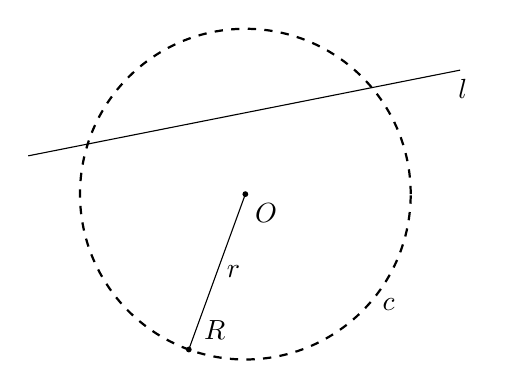
\begin{tikzpicture}[scale=.7]
\coordinate (O) at (0,0);
\node at (2.6,-2) {$c$};
\draw[thick,dashed] (O) circle[radius=3cm];
\fill (O) node[below right] {$O$} circle[radius=1.5pt];
\draw (O) -- node[right] {$r$} ++(-110:3cm) coordinate (R);
\fill (R) circle[radius=1.5pt] node[above right,xshift=2pt] {$R$};
\draw (O) +(170:4cm) -- node[below, near end,xshift=40pt,yshift=8pt] {$l$} ++(30:4.5cm);
\end{tikzpicture}
\end{center}
לפי משפט~%
\ref{thm.perpendicular}
ניתן לבנות אנך ממרכז המעגל
$O$
לקו
$l$.
סמנו ב-%
$M$
את נקודת החיתוך של
$l$
עם האנך. 
$M$
חוצה של המיתר 
$\overline{XY}$,
כאשר 
$X,Y$
הן נקודות החיתוך של הקו עם המעגל. 
סמנו ב-%
$2s$
את אורך המיתר. שימו לב שבאיור
$s,X,Y$
הם רק הגדרות וטרם בנינו את נקודות החיתוך.
\begin{center}

\begin{tikzpicture}[scale=.7]
\coordinate (O) at (0,0);
\node at (2.6,-2) {$c$};
\draw[thick,dashed,name path=circle] (O) circle[radius=3cm];
\fill (O) node[below right] {$O$} circle[radius=1.5pt];
\draw (O) -- node[right] {$r$} ++(-110:3cm) coordinate (R);
\fill (R) node[above right,xshift=2pt] {$R$} circle[radius=1.5pt];
\draw[name path=l] (O) ++(170:4cm) -- node[below, near end,xshift=40pt,yshift=12pt] {$l$} ++(20:8cm);
\path[name intersections={of=circle and l,by={Y,X}}];
\fill (X) node[above left] {$X$} circle[radius=1.5pt];
\fill (Y) node[above right,yshift=2pt] {$Y$} circle[radius=1.5pt];
\draw (O) -- node[below] {$r$} (X);
\path (X) -- ($(X)!.5!(Y)$) coordinate (M);
\fill (M) node[above] {$M$} circle[radius=1.5pt];
\draw (O) -- node[right] {$t$} (M);
\path (X) -- node[above] {$s$} (M);
\path (M) -- node[above] {$s$} (Y);
\draw (O) ++(170:4cm) -- ++(20:3.1cm) -- ++(-70:10pt) -- ++(20:10pt);
\end{tikzpicture}
\end{center}
$\triangle OMX$
הוא מעגל ישר-זווית ולכן
$s^2=r^2-t^2=(r+t)(r-t)$.
$r$
נתון כרדיוס המעגל ו-%
$t$
הוגדר כאורך של
$\overline{OM}$.
לפי משפט~%
\ref{thm.angle}
ניתן לבנות קטעי קו באורך
$r$
מהנקודה 
$O$
בשני הכיוונים
$\overline{MO}$
ו-%
$\overline{OM}$.
התוצאה היא שני קטעי קו שאורכם
$r+t,r-t$.

לפי משפט~%
\ref{thm.root}
ניתן לבנות קטע קו באורך
$s=\sqrt{(r+t)(r-t)}$.
שוב לפי משפט~%
\ref{thm.angle},
ניתן לבנות קטעי קו באורך 
$s$
על הקו הנתון
$l$
מהנקודה
$M$
בשני הכיוונים. הקצה השני של כל אחד מקטעי הקו האלה הוא נקודת חיתוך של 
$l$
עם המעגל.
\qed

%%%%%%%%%%%%%%%%%%%%%%%%%%%%%%%%%%%%%%%%%%%%%%%%%%%%%%%%%%%%%%%

\selectlanguage{hebrew}


\section{%
בניית נקודות החיתוך של שני מעגלים%
}\label{s.circle-circle}

\begin{theorem}\label{thm.two-circles}\mbox{}\\
נתונים שני מעגלים עם מרכזים
$O_1,O_2$
ורדיוסים
$r_1,r_2$.
ניתן לבנות את נקודות החיתוך שלהם
$X,Y$.
\end{theorem}
\textbf{הוכחה:}
בנו את קטע הקו
$\overline{O_1O_2}$
המחבר את שני המרכזים. סמנו את אורכו ב-%
$t$.
\begin{center}

\begin{tikzpicture}[scale=1.2]
\coordinate (O1) at (0,0);
\coordinate (O2) at (2.5,0);
\fill (O1) node[below left] {$O_1$} circle[radius=1.5pt];
\fill (O2) node[below right] {$O_2$} circle[radius=1.5pt];
\draw[thick,dashed,name path=circle1] (O1) circle[radius=2cm];
\draw[thick,dashed,name path=circle2] (O2) circle[radius=1.6cm];
\path [name intersections={of=circle1 and circle2,by={X,Y}}];
\draw (O1) -- node[above] {$r_1$} ++(160:2cm);
\draw (O2) -- node[above] {$r_2$} ++(30:1.6cm);
\fill (O1) ++(160:2cm) circle[radius=1.5pt];
\fill (O2) ++(30:1.6cm) circle[radius=1.5pt];
\draw (O1) -- (O2);
\node at (-1.7,1.6) {$c_1$};
\node at (3.8,1.4) {$c_2$};
\draw[<->] (0,-1) -- node[fill=white] {$t$} (2.5,-1);
%\node at (6,0) {$t=O_1O_2$};
\end{tikzpicture}
\end{center}
סמנו ב-%
$A$
את נקודת החיתוך של
$\overline{O_1O_2}$
עם
$\overline{XY}$,
וסמנו את
$q=\overline{O_1A},x=\overline{XA}$.
טרם בנינו את הנקודה
$A$,
אבל אם נצליח לבנות את האורכים
$q,x$,
לפי משפט~% 
\ref{thm.angle}
נוכל לבנות את 
$A$
באורך
$q$
מהנקודה
$O_1$
לכיוון
$\overline{O_1O_2}$.
לפי משפט~%
\ref{thm.perpendicular}
ניתן לבנות את האנך ל-%
$\overline{O_1O_2}$
בנקודה
$A$,
ושוב לפי משפט~%
\ref{thm.angle}
ניתן לבנות קטעי קו באורך
$x$
מהנקודה
$A$
בשני הכיוונים לאורך האנך.
$X,Y$,
הקצות של קטעי הקו, הם נקודות החיתוך של שני המעגלים.
\begin{center}

\begin{tikzpicture}[scale=1.2]
\coordinate (O1) at (0,0);
\coordinate (O2) at (2.5,0);
\fill (O1) node[below left] {$O_1$} circle[radius=1.5pt];
\fill (O2) node[below right] {$O_2$} circle[radius=1.5pt];
\draw[thick,dashed,name path=circle1] (O1) circle[radius=2cm];
\draw[thick,dashed,name path=circle2] (O2) circle[radius=1.6cm];
\path [name intersections={of=circle1 and circle2,by={X,Y}}];
\fill (X) node[above,yshift=4pt] {$X$} circle[radius=1.5pt];
\fill (Y) node[below,yshift=-4pt] {$Y$} circle[radius=1.5pt];
\draw[thick,dashed] (O1) -- node[above,xshift=-4pt] {$r_1$} (X);
\draw[thick,dashed] (O2) -- node[above,xshift=4pt] {$r_2$} (X);
\draw[name path=oo] (O1) -- (O2);
\node at (-1.7,1.6) {$c_1$};
\node at (3.8,1.4) {$c_2$};
\draw[name path=xy] (X) -- (Y);
\path[name intersections={of=xy and oo,by={A}}];
\fill (A) node[below left] {$A$} circle[radius=1.5pt];
\path (O1) -- node[below,xshift=-2pt] {$q$} (A);
\path (X) -- node[left,yshift=-2pt] {$x$} (A);
\draw[<->] (0,-1) -- node[fill=white] {$t$} (2.5,-1);
\node at (6,.5) {$t=\overline{O_1O_2}$};
\node at (6,0) {$q=\overline{O_1A}$};
\node at (6,-.5) {$x=\overline{XA}$};
\end{tikzpicture}
\end{center}
\textbf{בניית האורך
$q$:}
בנו
$d=\sqrt{r_1^2+t^2}$, 
אורך היתר של משולש ישר-זווית מהאורכים הידועים
$r_1,t$:
על קו כלשהי במישור בנו קטע קו
$\overline{RS}$
באורך
$r_1$,
אחר כך בנו אנך ל-%
$\overline{RS}$
דרך
$R$,
ולבסוף בנו קטע קו
$\overline{RT}$
באורך 
$t$
מ-%
$R$
על האנך.

לפי משפט הקוסינוסים ב-%
$\triangle O_1O_2X$:

\begin{eqnarray*}
r_2^2 &=& t^2 + r_1^2 - 2r_1t\cos\angle XO_1O_2\\
\disfrac{q}{r_1}&=&\cos\angle O_1O_2X\\
r_2^2&=& t^2 + r_1^2 - 2tq\\
2tq &=& (r_1^2+t^2) - r_2^2\\
q&=&\disfrac{(d+r_2)(d-r_2)}{2t}\,.
\end{eqnarray*}


לפי משפט~%
\ref{thm.angle}
ניתן לבנות את האורכים האלה, ולפי משפט~%
\ref{thm.three-lines}
ניתן לבנות את
$q$
מהביטויים
$d+r_2,d-r_2,2t$.

\textbf{בניית האורך
$x$:}
$\triangle AO_1X$
הוא משולש ישר-זווית ולכן:
\[
x^2=r_1^2-q^2 =\sqrt{(r_1+q)(r_1-q)}\,.
\]
לפי משפט~%
\ref{thm.angle}
ניתן לבנות
$h =r_1+ q$
ו-%
$k= r_1 - q$,
ולפי משפט~%
\ref{thm.root}
ניתן לבנות
$x= \sqrt{hk}$. 

\selectlanguage{hebrew}


\subsection*{מקורות}
הפרק מבוסס על בעיה
$34$
ב-%
\L{\cite{dorrie1}}
שעובדה על ידי
\L{Michael Woltermann} \L{\cite{dorrie2}}. 
ברצוני להודות לו על הרשות להתשמש בעבודתו.


